\documentclass[a4paper,12pt]{article}
\hbadness=10000
\usepackage{geometry}
 \geometry{
 total={170mm,257mm},
 left=20mm,
 top=20mm,
 }
 \usepackage{wrapfig}
\usepackage{graphicx}
\usepackage{listings}
\lstdefinelanguage{TypeScript}{
    keywords={const, let, function, if, else, return, class, extends, super, import, export, new, public, private, protected, True, False},
    morekeywords={[2]true, false, null, undefined},
    morecomment=[l]{//},
    morecomment=[s]{/*}{*/},
    morestring=[b]',
    morestring=[b]"
}
\lstset{
    language=TypeScript,
    basicstyle=\ttfamily\footnotesize,
    keywordstyle=\color{blue},
    keywordstyle={[2]\color{orange}},
    commentstyle=\color{gray},
    stringstyle=\color{red},
    frame=single,
    breaklines=true,
    showspaces=false,
    showtabs=false,
    captionpos=b,
    columns=flexible,
    numbers=left,
    numberstyle=\tiny\color{gray},
}
\usepackage{tocloft}
\usepackage{tikz}
\usetikzlibrary{positioning, arrows.meta}

\tikzset{
  process/.style={
    rectangle, draw=black, fill=blue!10, rounded corners, minimum width=3.5cm, minimum height=2cm, align=center
  },
  testbereich/.style={
    rectangle, draw=orange!80!black, fill=orange!10, rounded corners, minimum width=3.5cm, minimum height=1.2cm, align=center
  },
  arrow/.style={
    -{Latex[length=3mm]}, thick,
  }
}

\usepackage{placeins}
\usepackage{xcolor}
\usepackage{titling}
\usepackage{float}
\usepackage{fancyhdr}
\usepackage{hyperref}
\usepackage{lmodern}
\usepackage[T1]{fontenc}
\usepackage{url}
\usepackage[none]{hyphenat}
\usepackage{setspace}  % Für den Zeilenabstand
\usepackage{fontspec}
\usepackage{ragged2e}  % Für Blocksatz
\renewcommand{\normalsize}{\fontsize{12}{14}\selectfont} 
\renewcommand{\listfigurename}{}
\renewcommand{\contentsname}{Inhaltsverzeichnis}
\renewcommand{\refname}{Literaturverzeichnis} 
\renewcommand{\figurename}{} % Entfernt das Wort "Abbildung" vor Bildern% 
\setlength{\cftbeforesecskip}{4pt} 
% Kopfzeilen-Einstellungen%
\renewcommand{\baselinestretch}{1.5} \pagestyle{fancy}
\fancyhf{} 
\setlength{\textheight}{240mm}  % Reduziert die Höhe des Textbereichs
\setlength{\footskip}{20mm} 
\renewcommand{\headrulewidth}{0pt}
\setlength{\headheight}{45.97pt}  
\fancyhead[L]{
\includegraphics[width=4cm]{images/LHsystemsLogo.png}}  
\fancyhead[R]{
\includegraphics[width=3.5cm]{images/DHBW-Logo.svg.png}} 

\begin{document}
 \justifying  
 \sloppy

\pagenumbering{gobble}

\setlength{\topskip}{60pt}  

% Titel
\begin{center}
    \setlength{\baselineskip}{18pt}
    {\large \textbf{Visualisierung dynamischer Flugrestriktionen in der Applikation Very Versatile Visualizer}} \\[0.4cm]
\end{center}

\vspace{1cm}  

% Studiengang & Hochschule
\begin{center}
    \setlength{\baselineskip}{18pt}
    im Studiengang \\
    {\color{red} \textbf{Angewandte Informatik}}\\
    an der Dualen Hochschule Baden-Württemberg Mannheim
\end{center}

\vspace{1.5cm}

% Autor
\begin{center}
    \setlength{\baselineskip}{18pt}
    von \\
    {\color{red} \textbf{Alexander Dugaj}}
\end{center}

\vspace{5cm}

% Weitere Informationen
\begin{flushleft}
    \begin{tabular}{l l}
        Abgabedatum:          & {\color{red} 28.08.2025} \\[0.3cm]
        Bearbeitungszeitraum: & {\color{red} 24 Wochen}  \\[0.3cm]
        Matrikelnummer, Kurs: & {\color{red} 1579702, Tinf23Ai2} \\[0.3cm]
        Ausbildungsfirma:     & {\color{red} Lufthansa Systems, Raunheim} \\[0.3cm]
        Betrieblicher Betreuer: & {\color{red} Jonas Sperling} \\[1cm]
    \end{tabular}
\end{flushleft}

\vfill

% Unterschrift
\begin{flushleft}
    \rule{6cm}{0.4pt} \\ 
    Unterschrift Betreuer
\end{flushleft}

\newpage

\section*{Erklärung}
\addcontentsline{toc}{section}{Erklärung}

\begin{center}
    \fcolorbox{black}{lightgray}{  
        \parbox{0.95\textwidth}{
            \textbf{Erklärung} \\[1em]
            Ich versichere hiermit, dass ich meine Projektarbeit mit dem Thema "Visualisierung dynamischer Flugrestriktionen in der Applikation Very Versatile Visualizer" selbstständig verfasst und keine anderen als die angegebenen Quellen und Hilfsmittel benutzt habe. Ich versichere zudem, dass die eingereichte elektronische Fassung mit der gedruckten Fassung übereinstimmt. \\[2em]
        
            \rule{5cm}{0.4pt} \hspace{4cm} \rule{5cm}{0.4pt} \\[1em]
            
            \hspace{0cm} Ort, Datum \hspace{6.75cm} Unterschrift}}
\end{center}

\newpage

\section*{Abstrakt}
\addcontentsline{toc}{section}{Abstrakt}
\newpage
\section*{Abstract}
\addcontentsline{toc}{section}{Abstract}

\newpage
\section*{Glossar}
\addcontentsline{toc}{section}{Glossar}

\newpage
\section*{Abbildungsverzeichnis}
\addcontentsline{toc}{section}{Abbildungsverzeichnis}

\listoffigures  

\newpage
\tableofcontents

\newpage
\pagenumbering{arabic}
\setcounter{page}{1}  % Startet die Nummerierung neu ab 1
\fancyfoot[C]{\thepage}
\section{Einleitung}
Die zivile Luftfahrt ist zunehmend von dynamischen Prozessen und komplexen Regeln geprägt. Diese regeln ständig einzuhalten in nicht nur schwer, sondern kann auch sehr schnell teuer werden, wenn man dies uneffizient macht. Es gibt verschiedene Arten von Regeln in der Flugbranche. Zu diesen gehören auch die Flugrestriktionen. Diese Flugrestriktionen sind spezielle Regeln die ein Flug von Start bis Landung einhalten muss. Zum einen haben diese sicherheitsrelevante Hintergründe aber zum anderen sind es einfach regeln wie zum Beispiel aufgrund des Militärs. Die Herauforderung ist diese Regeln bestmöglich in den Flugrouten zu beachten und vorallem einzuhalten. \\
Die Abteilung Lido Flight Planning arbeitet konkret an solchen Flugoptimierungen. Während man eine Flugroute plant muss man wie bereits erwähnt auf viele regeln achten. Damit auch alle Restriktionen, die auf eine Flugroute fallen, erfüllt sind. Diese Daten werden bei uns Intern in disjunktive Normalformen umgeformt, damit man diese leichter interpretieren kann. Um eine Flugroute jetzt am besten planen kann, müssen neben vielen anderen Aspekten auch die Restriktionen verständlich sein.
\subsection{Problemstellung}
Flugretriktionen sind wichtig einzuhalten. Aber dafür muss man diese verstehen und weiter nutzen können, aber leider können Retsriktionen belibig lange und somit auch belibieg komplex werden. Diese Restriktionen liegen als reine roh daten in anderen Applikationen. Bis man diese Restriktion vollständig verstanden hat kann es einige Zeit dauern. Deshalb werden diese bei uns in disjunktive Normalformen umgewandelt. Damit muss ein Flug nurnoch ein Fall erfüllen, damit diese Flugrestriktion gilt. Aber das Problem ist die Disjunktive Normalform kann beliebig lang werden und somit wird auch das einsehen und verstehen immer schwerer. Wenn die Einsicht immer wieder länger dauert, verliert das Team viel Zeit für das Verständnis der Restriktionen und nicht für die Flugplanung oder ähniches. Außerdem würde im Falle eines Fehlers in der Flugroute nur schwer herausgefunden werden, woran es liegt. Mit dieser Arbeit könnte es als zusätzliche Hilfetool genutzt werden. Aktuell fehlt eine intuitive Möglichkeit, Flugrestriktionen vollständig und visuell verständlich darzustellen. Zwar existiert bereits eine erste Lösung in einer separaten Applikation, jedoch ist diese funktional eingeschränkt und ermöglicht nur den Zugriff auf einen kleinen Teil der verfügbaren Restriktionsdaten. Besonders bei der gleichzeitigen Betrachtung von Flugroute und Restriktionen entsteht dadurch ein hoher Aufwand. Das kostet nicht nur Zeit, sondern erhöht auch das Risiko von Planungsfehlern und ineffizienten Entscheidungen im Flugroutenmanagement.
\begin{figure}[H]
    \centering
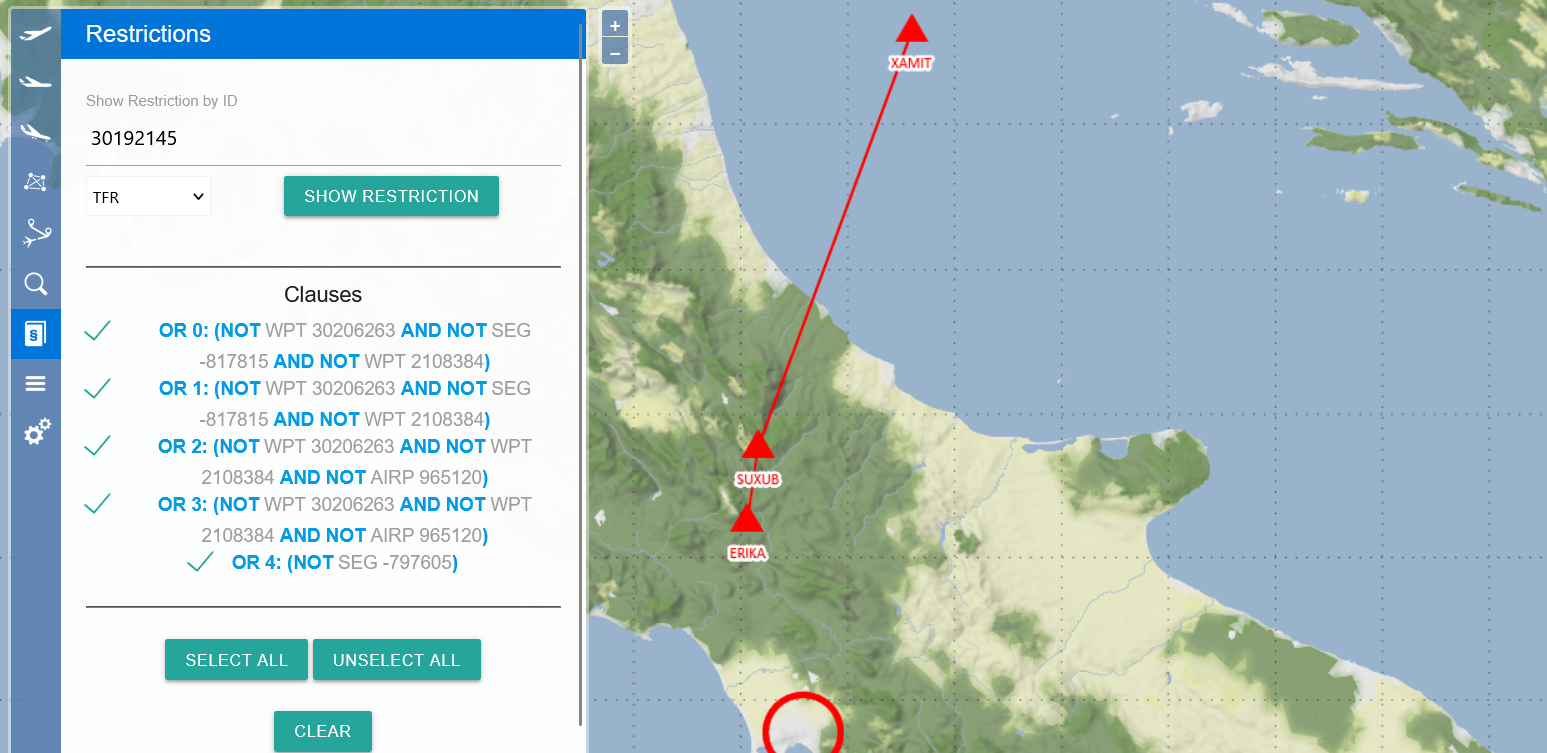
\includegraphics[width=1\textwidth]{images/Bespiel1.png}
\caption{Bestehende Darstellung}
\end{figure}
Abbildung 1 ist ein Auschnitt aus der bestehnden Lösung. LIEBER AN ANFANG DES HAUPTTEILES
\subsection{Ziel}
Damit die Flugrestriktion ganz einfach und schnell verstanden werden und zudem weiterverwendet verden können, ist das Ziel dieser Arbeit diese Restriktion in der Applikation vvv in einem eigenen Bereich anzuzeigen, damit man auf einem Blick alles einsehen kann, was man braucht. Das soll sicherstellen, das die Nutzer sofort auf einem Blick das sehen was sie brauchen und somit ein Menge Zeit sparen. Ausserdem sollen nicht nur die Restriktion als disjunktive Normalform gezeigt werden, sondern auch sämtliche zusätzliche Informationen anzeigen. Außerdem sollen diese Restriktion auf der in der Applikation verfügbaren Karte angezeigt werden. Damit kann man die restriktion nicht nur logisch anhand der dnf sehen, sondern auch praktisch an der Karte verstehen.  Meine Lösung soll von Nutzer aus der Kundensicht genutzt werden aber auch aus der Entwicklersicht.
\subsection{Aufbau der Arbeit}
\newpage
\section{Grundlagen}
\subsection{Theoretische Grundlagen}
\subsubsection{Flugrestriktionen}
Flugrestriktionen sind einschränkende Vorgaben, die den Luftverkehr in bestimmten geografischen Bereichen oder unter bestimmten Bedingungen regeln. Sie dienen in erster Linie der Sicherheit, Effizienz und Koordination im nationalen und internationalen Luftraum. Solche Restriktionen legen beispielsweise fest, wo, wann und wie ein Luftfahrzeug bestimmte Zonen durchfliegen darf oder muss. Die Einschränkungen können sich auf Höhenbereiche, Zeiträume, Flugrichtungen oder spezifische Regeln beziehen. Besonders häufig wirken sich Flugrestriktionen auf sogenannte Wegpunkte aus. Dabei handelt es sich um geografisch exakt definierte Koordinaten im dreidimensionalen Raum, die zur Navigation und Strukturierung von Flugrouten dienen. Mehrere solcher Wegpunkte lassen sich zu sogenannten Segmenten verketten, die gemeinsam einen Abschnitt einer geplanten Flugstrecke bilden. Darüber hinaus gelten für definierte Lufträume (Flugbereiche oder Airspaces) häufig spezielle Einschränkungen. Auch für Flughäfen existieren restriktive Vorschriften, etwa im Zusammenhang mit Anflugverfahren, wie soll der Flughafen genutzt werden, temporären Sperrungen oder militärischer Nutzung. Das sind vier der am meisten vorkommenden Typen bei dieser Abreit, und auf denen sollte auch der Fokus liegen. ABer trotzdem gibt es natürlich auch weitere. \\
In der Praxis sind zwei Arten von Flugrestriktionen besonders relevant. zum einen gibt es die TFRs (Temporary Flight Restrictions) und zum anderen die NOTAMs (Notice to Airmen). Temporäre Flugbeschränkungen sind zeitlich begrenzte Luftraumbeschränkungen, die von der US-Luftfahrtbehörde Federal Aviation Administation (FAA) eingerichtet werden, um Sicherheit, Schutz oder Privatsphäre zu gewährleisten. Solche Beschränkungen treten zum Beispiel bei Naturkatastrophen, dem Transport von Staatsgästen oder Waldbränden in Kraft und dürfen ohne Genehmigung nicht überflogen werden. Die entsprechenden Informationen werden über das NOTAM-System veröffentlicht (vgl.\cite{quelle1}). NOTAMs sind offizielle Mitteilungen der Luftfahrtbehörde, die kurzfristige Änderungen, Einschränkungen oder Gefahren im Luftverkehr bekannt geben. Sie dienen der Information von Pilotinnen und Flugplanerinnen über sicherheitsrelevante Luftraumänderungen (vgl.\cite{quelle1}).
 \subsubsection{Disjunktive Normalform}
 \subsubsection{Flugrestriktionen in Lido Flight}

Die Abteilung, in der diese Arbeit erfolgt ist Lido Flight Planning Software. Diese... \\
Diese wandelt die Flugrestriktionen in Disjunktive Normalforemn um. Disjunktive Normalforemn 
\subsection{Teschnische Grundlagen}
\subsubsection{Very Versatile Visualizer (unsere appliaktion)}
\subsubsection{Svelte}
\subsubsection{Java Spring Boot}
\subsubsection{Figma}
\subsubsection{Swagger UI}
\newpage
\section{Entwicklungsprozess}
\begin{figure}[H]
    \centering
        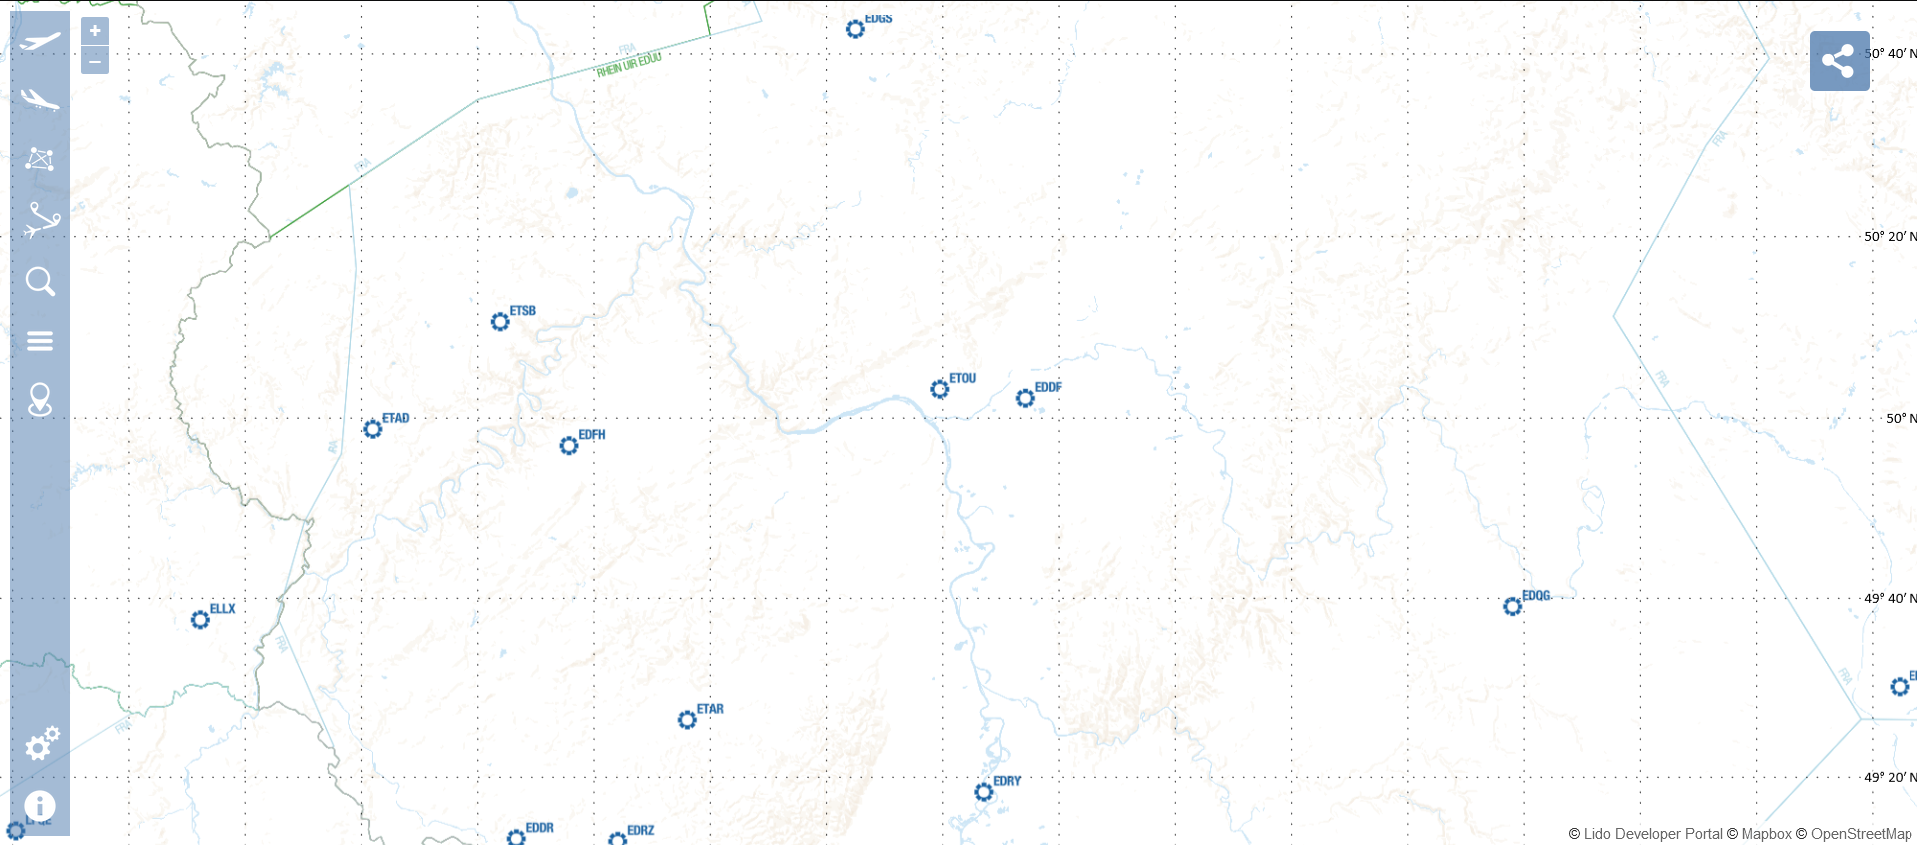
\includegraphics[width=1\textwidth]{images/VVVVorEntwicklung.png}
\caption{VVV vor der Entwicklung}
\end{figure}
\begin{wrapfigure}{l}{0.4\textwidth}
    \centering
    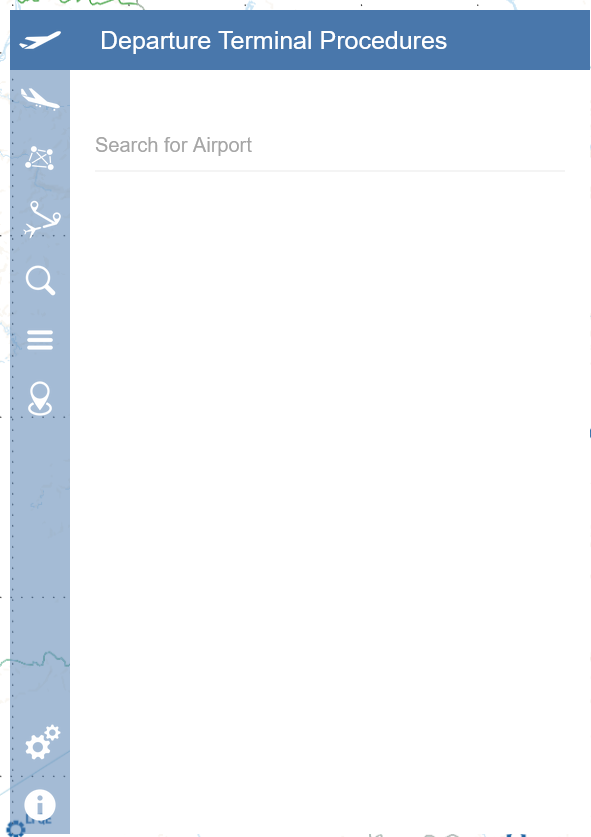
\includegraphics[width=0.35\textwidth]{images/AirportTab.png}
    \caption{Airport Register}
\end{wrapfigure}
In dieser Abbildung sieht man die Applikation VVV vor der Entwicklung der Restriktions Funktion. Im Zentrum ist die Karte zu sehen und auf der linken Seite sieht man die Registerkartenauswahl. Das sind jeweils verschieden Funktionalitäten wie zum Beispiel das erste Symbol, das abhebende Flugzeug. Nachdem auf das Symbol geklickt wurde, öffnet sich ein Seitenleiste, mit einem Suchfeld für Flughäfen. Dieses design ist bei jedem Register identsich, da man immer die selbe Komponente nutzt. 
\\\\\\
\subsection{Anforderungen}
Bevor die Entwicklung begonnen werden kann, ist es wichtig, die funktionalen Anforderungen an diean die geplante Visualisierung zu definieren. Diese Anforderungen dienen als Grundlage für die Entwicklung und helfen, den Fokus auf die wesentlichen Aspekte zu legen.\\
Die zentrale Anforderung besteht darin, dass Flugrestriktionen gezielt durch Eingabe einer eindeutigen ID sowie eines zugehörigen Restriktionstyps gesucht werden können. Bei einer gültigen Eingabe soll die entsprechende Restriktion in Form einer disjunktiven Normalform (DNF) angezeigt werden. Sollte die ID nicht existieren oder die Eingabe ungültig sein, muss eine entsprechende Fehlermeldung erscheinen. Die Darstellung der DNF soll dabei so aufbereitet sein, dass sie für Nutzerinnen und Nutzer leicht verständlich ist. Das bedeutet, dass die einzelnen Bedingungen und Klauseln klar erkennbar sind und insbesondere, ob ein Literal negiert ist \(( \neg A )\) oder nicht \(( A )\). Die Herausforderung hierbei ist, dass die DNF beliebig lang sein kann. Jede Einzelne Klausel kann ebenfalls eine beliebige Anzahl an Literalen haben. Solche Fälle sollen dementsrpechend übersichtlich dargestellt werden, um eine klare Lesbarkeit zu gewährleisten.
Eine weitere wesentliche Anforderung ist die eindeutige Erkennung des Literaltyps. Es existieren eine Menge an verschiedenen Literaltypen, aber es soll in erster Linie zwischen den wichtigsten Literaltypen klar unterschieden werden können. Diese sollen visuell klar voneinander unterscheidbar sein, sodass Nutzerinnen und Nutzer auf einen Blick erkennen können, um welche Art von Element es sich jeweils handelt. Diese Literaltypen kommen am häufigsten vor. Darüber hinaus enthält jeder Literaltyp zusätzliche kontextspezifische Informationen, die für das Verständnis der Flugrestriktion von Bedeutung sind. Wie Bei Flughäfen ist beispielsweise zu unterscheiden, ob es sich um den Abflug- oder den Ankunftsflughafen handelt. Solche Zusatzinformationen sollen innerhalb der Visualisierung ebenfalls deutlich und übersichtlich dargestellt werden. Schließlich gibt es bei der Nutzung der Funktionalität Variationen. So bevorzugen manche Personen bei der Arbeit mit den Literaltypen die Anzeige der eindeutigen ID, während andere lieber den ausgeschriebenen Namen verwenden. Deshalb soll ebenfalls eine Funktionlität hinzufügt werden, bei der die Nutzer selber entscheiden können, welche Anzeige sie grade benötigen. \\
Nachdem die DNF verständlich visualsiert ist, sollen die relevanten  Literalentypen auf der Karte dargestellt werden. Die Herausforderung besteht darin, eine Überladung der Karte zu vermeiden und gleichzeitig alle entscheidenden Informationen auf einen Blick verfügbar zu machen. Zudem soll sichergestellt werden das die Karte genau das anzeigt, was die restriktion ausdrücken will. Das bedeutet es muss sichergesetllt werden, dass auch negierte Literale anders gekennzeichnet werden wie positive Literale. So muss beispielsweise in einer Restriktion wie \[( A \land B) \lor (A \land B \land C)\] anders dargestellt werden, als \[( \neg A \land B) \lor (\neg A \land B \land C).\] Der Hintergrund hier ist, das wenn eine Restriktion ein Literal \(A\) nur als positiv hat, bedeutet es, man muss dieses Element befliegen um diese Restrikiton zu erfüllen. Andersrum sollte ein Literal \(A\) nur negiert vorkommen bedeutet dies, man darf diese Elemente unter keinem Umstand befliegen. Sollte man aber einen Fall wie \[(\neg A \land B) \lor (A \land B \land \neg C)\] haben, so muss man noch darstellen das Literal \(A\) in einer Klausel beflogen werden muss, aber in einer anderen nicht. Die Karte soll somit diese Logik klar darstellen, damit man diese Information auf einem Blick hat und ggf. weiter verwednen kann. \\
Eine wichtige nicht-funktionale Anforderung betrifft das visuelle Erscheinungsbild der Anwendung. Der Very Versatile Visualizer (VVV) zeichnet sich durch ein modernes, übersichtliches und benutzerfreundliches Design aus. Deshalb sollten die hier erstelleten Funktionaitäten sich in das bestehende Designkonzept integrieren. Das bedeutet, dass sich die neuen Darstellungen und Interaktionen visuell und strukturell an den bereits vorhandenen Registerinhalten orientieren und keine stilistischen Brüche erzeugen.
\[optionale\space Features\space erwaehnen ?\]
\subsection{Design}
\subsection{Disjunktive Normalf visualisieren}
\subsection{Karten Elemnte Konfigurieren}
\newpage
\section{Bewertung der Ergebnisse}
\newpage
\section{Kritische Reflexion}


\newpage
\pagenumbering{gobble}
\begin{thebibliography}{9}  % Die Zahl bestimmt die Breite der Nummerierung
\bibitem{quelle1}
Blade Urban Air Mobility, 2024, Temporary Flight Restrictions (TFR), https://www.blade.com/TFR, abgerufen am 18.07.2025


\end{thebibliography}
\addcontentsline{toc}{section}{Literaturverzeichnis}

\end{document}